\documentclass{ximera}

\newcommand{\RR}{\mathbb R}
\renewcommand{\d}{\,d}
\newcommand{\dd}[2][]{\frac{d #1}{d #2}}
\renewcommand{\l}{\ell}
\newcommand{\ddx}{\frac{d}{dx}}
\newcommand{\dfn}{\textbf}
\newcommand{\eval}[1]{\bigg[ #1 \bigg]}


\outcome{Understand the definiton of a multiple integral.}

\outcome{Use iterated integrals to compute multiple integrals.}

\outcome{Apply Fubini's Theorem.}

\title[Dig-In:]{Integrals over trivial regions}

\begin{document}
\begin{abstract}
  We study integrals over basic regions.
\end{abstract}
\maketitle

As we journey through calculus again, we are now ready for integrals.
Instead of integrating over an interval like $[a,b]$ we now integrate
over regions like this
\[
R = \{(x,y):\text{$x$ and $y$ satisfy some property}\}
\]
in particular, in this section we will only consider rectangles and
boxes, and this is what we mean by ``trivial'' regions. Here a
rectangle is defined as:
\[
R = \{(x,y):\text{$a\le x\le b$ and $c\le y\le d$}\}
\]
A box is defined as:
\[
R = \{(x,y):\text{$a\le x\le b$, $c\le y\le d$, and $p\le q$}\}
\]
Let's get to work!


\section{Double integrals}

Suppose you have a function $F:\R^2\to\R$. A graph of this function is
a surface in $\R^3$. For example:
\begin{image}
  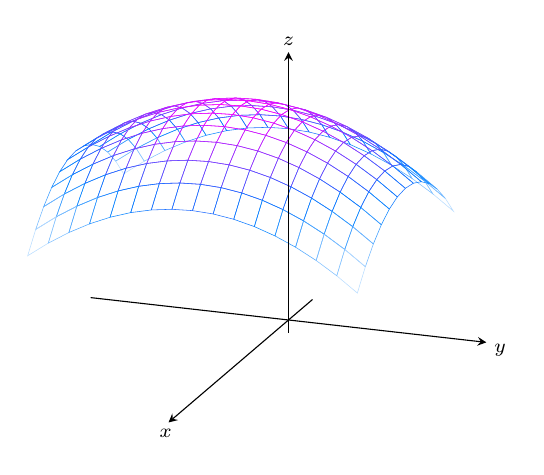
\begin{tikzpicture}
    \begin{axis}%
      [ tick label style={font=\scriptsize},axis on top,
	axis lines=center,
	view={110}{25},
	name=myplot,
	xtick=\empty,
        ytick=\empty,
        ztick=\empty,
	ymin=-1.2,ymax=1.2,
	xmin=-.5,xmax=2.5,
	zmin=-.1, zmax=2.1,
	every axis x label/.style={at={(axis cs:\pgfkeysvalueof{/pgfplots/xmax},0,0)},xshift=-1pt,yshift=-4pt},
	xlabel={\scriptsize $x$},
	every axis y label/.style={at={(axis cs:0,\pgfkeysvalueof{/pgfplots/ymax},0)},xshift=5pt,yshift=-3pt},
	ylabel={\scriptsize $y$},
	every axis z label/.style={at={(axis cs:0,0,\pgfkeysvalueof{/pgfplots/zmax})},xshift=0pt,yshift=4pt},
	zlabel={\scriptsize $z$},
        colormap/cool,
      ]
      %% Surface %% 12 x 16
      \addplot3[domain=0:2,y domain=-1:1,mesh,samples=13,samples y=17,very thin,z buffer=sort] {-.5*(x-1)^2-.5*(y)^2+2};
    \end{axis}
  \end{tikzpicture}
\end{image}

We are interested in the ``signed volume'' or ``net volume'' between
this surface and the $(x,y)$-plane. This means that the space above
the $(x,y)$ plane under $F$ will have a positive volume.  Space above
$F$ and under the $(x,y)$-plane will have a ``negative'' volume. This
is similar to the notion of ``signed area'' used before.  If we want
to compute the signed volume of a surface defined by $F$ over a
rectangular region, say the rectangle defined by
\[
R = \{(x,y):\text{$a\le x\le b$ and $c\le y\le d$}\}
\]
we break $R$ into $n$ slices parallel to the $x$-axis, and $m$ slices
parallel to the $y$-axis. This allows us to consider boxes of
dimension
\[
\underbrace{F(x_i^*,y_j^*)}_{\text{height}}\times\underbrace{\left(\frac{b-a}{m}\right)}_{\Delta x}\times \underbrace{\left(\frac{d-c}{n}\right)}_{\Delta y}
\]
where $(x_i^*,y_j^*)$ is a point in $(i,j)$-rectangle:
\begin{image}
  \begin{tikzpicture}
    \begin{axis}%
      [tick label style={font=\scriptsize},axis on top,
	axis lines=center,
	view={110}{25},
	name=myplot,
        xtick=\empty,
        ytick=\empty,
        ztick=\empty,
	ymin=-1.2,ymax=1.2,
	xmin=-.5,xmax=2.5,
	zmin=-.1, zmax=2.1,
	every axis x label/.style={at={(axis cs:\pgfkeysvalueof{/pgfplots/xmax},0,0)},xshift=-1pt,yshift=-4pt},
	xlabel={\scriptsize $x$},
	every axis y label/.style={at={(axis cs:0,\pgfkeysvalueof{/pgfplots/ymax},0)},xshift=5pt,yshift=-3pt},
	ylabel={\scriptsize $y$},
	every axis z label/.style={at={(axis cs:0,0,\pgfkeysvalueof{/pgfplots/zmax})},xshift=0pt,yshift=4pt},
	zlabel={\scriptsize $z$},
        colormap/cool,clip=false,
      ]
      %% 12 lines
      \pgfplotsinvokeforeach{0,0.1667,...,2}{
        \draw[gray] (axis cs: #1,-1,0) -- (axis cs: #1 , 1,0);
      }

      %% 16 lines
      \pgfplotsinvokeforeach{-1,-.875,...,1}{
        \draw[gray] (axis cs: 0,#1,0) -- (axis cs: 2 ,#1,0);
      }


      %% \pgfplotsinvokeforeach{-1,-.875,...,1}{
      %%   \addplot3[domain=0:2,y domain=-1:1,mesh,samples=13,samples
      %%     y=17,very thin,z buffer=sort] {-.5*(x-1)^2-.5*(y)^2+2};
      %%   }

      

      %% Box vol
      \draw [gray,thick]
      (axis cs: 1.833,.25,0) --
      (axis cs: 1.833,.375,0) --
      (axis cs: 1.833,.375,1.665) --
      (axis cs: 1.833,.25,1.665) --
      (axis cs: 1.833,.25,0);

      \draw [gray,thick]
      (axis cs: 1.833,.375,0) --
      (axis cs: 1.833,.375,1.665) --
      (axis cs: 1.667,.375,1.665) --
      (axis cs: 1.667,.375,0) --
      (axis cs: 1.833,.375,0);

      \draw [gray,thick]
      (axis cs: 1.667,.375,1.665) --
      (axis cs: 1.667,.25,1.665) --
      (axis cs: 1.833,.25,1.665);

      %% Surface %% 12 x 16
      \addplot3[domain=0:2,y domain=-1:1,mesh,samples=13,samples y=17,very thin,z buffer=sort] {-.5*(x-1)^2-.5*(y)^2+2};

      %% Surface curves
      \addplot3[domain=0:2,%fill=white,
        penColor,very thick,samples=13,samples y=0] (
               {x},
               {1},
               {-.5*(x-1)^2-.5*(1)^2+2});

      \addplot3[domain=0:.5,%fill=white,
        penColor,very thick,dashed,samples=13,samples y=0] (
               {x},
               {-1},
               {-.5*(x-1)^2-.5*(-1)^2+2});

      \addplot3[domain=.5:2,%fill=white,
        penColor,very thick,samples=13,samples y=0] (
               {x},
               {-1},
               {-.5*(x-1)^2-.5*(-1)^2+2});

      \addplot3[domain=-1:1,%fill=white,
        penColor,very thick,samples=13,samples y=18] (
               {2},
               {y},
               {-.5*(2-1)^2-.5*(y)^2+2});

      \addplot3[domain=-1:.8,%fill=white,
        dashed,penColor,very thick,samples=13,samples y=18] (
               {0},
               {y},
               {-.5*(0-1)^2-.5*(y)^2+2});

      \addplot3[domain=.75:1,%fill=white,
        penColor,very thick,samples=13,samples y=18] (
               {0},
               {y},
               {-.5*(0-1)^2-.5*(y)^2+2});

      %% %% dxdydz         
      %% \draw [penColor, thick]
      %% (axis cs: 1.667,.25,1.746) --(axis cs: 1.667,.375,1.71) --
      %% (axis cs: 1.833,.375,1.583) --(axis cs: 1.833,.25,1.621) --
      %% (axis cs: 1.667,.25,1.746) -- (axis cs: 1.667,.375,1.71);
      
      \draw[decoration={brace,raise=.1cm},decorate,thin] (axis cs:0,-1,0)--(axis cs: 0,1,0);
      \node at (axis cs: -.6,-.1,0) {\scriptsize$n$};
      
      \draw[decoration={brace,mirror,raise=.1cm},decorate,thin] (axis cs:0,-1,0)--(axis cs: 2,-1,0);
      \node at (axis cs: .7,-1.25,0) {\scriptsize$m$};
      
      \draw[->,thin] (axis cs:1.75,1.2,0)--(axis cs: 1.75,.375,0);
      \node at (axis cs: 1.75,1.3,0) {\scriptsize$\Delta x$};

      \draw[->,thin] (axis cs:2.2,.3125,0)--(axis cs: 1.833,.3125,0);
      \node at (axis cs: 2.4,.3125,0) {\scriptsize$\Delta y$};

      \draw[decoration={brace,mirror,raise=.1cm},decorate,thin] (axis cs: 1.833,.25,1.665) -- (axis cs: 1.833,.25,0);
      \node[above left] at (axis cs: 1.833,.2,.8) {\scriptsize$ F(x_i^*,y_j^*)$};
    \end{axis}
  \end{tikzpicture}
\end{image}

Computing the volume of each of these boxes approximates and summing them together
\[
\sum_{j=1}^n\sum_{i=1}^m F(x^*_i,y^*_j)\Delta x\Delta y
\]
approximates the signed volume enclosed by the surface: 

\begin{image}
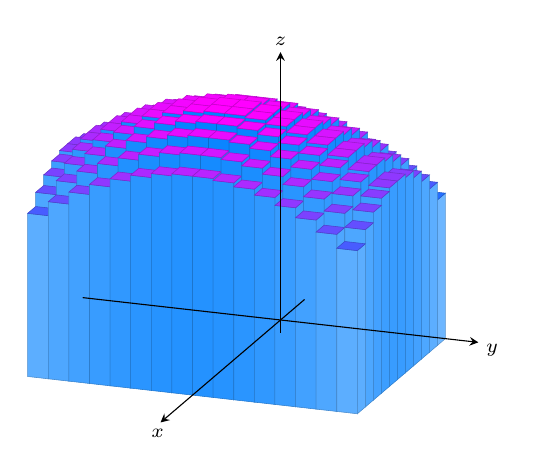
\begin{tikzpicture}
    \begin{axis}%
      [tick label style={font=\scriptsize},axis on top,
	axis lines=center,
	view={110}{25},
	name=myplot,
	xtick=\empty,
	ytick=\empty,
     ztick=\empty,
	ymin=-1.2,ymax=1.2,
	xmin=-.5,xmax=2.5,
	zmin=-.1, zmax=2.1,
	every axis x label/.style={at={(axis cs:\pgfkeysvalueof{/pgfplots/xmax},0,0)},xshift=-1pt,yshift=-4pt},
	xlabel={\scriptsize $x$},
	every axis y label/.style={at={(axis cs:0,\pgfkeysvalueof{/pgfplots/ymax},0)},xshift=5pt,yshift=-3pt},
	ylabel={\scriptsize $y$},
	every axis z label/.style={at={(axis cs:0,0,\pgfkeysvalueof{/pgfplots/zmax})},xshift=0pt,yshift=4pt},
	zlabel={\scriptsize $z$},
        colormap/cool,
      ]
      \foreach \j in {0,.125,...,1.875}{
       \foreach \i in {0,0.1667,...,1.8333}{        
        %% RIGHT SIDE
        \addplot3[opacity=1,surf,domain=0+\i:.1667+\i,y domain=0:{-.5*(((0+\i +.1667+\i )/2)-1)^2-.5*((-1+\j-.875+\j)/2)^2+2},samples=2,samples y=2,very thin,z buffer=sort] (x,-.875+\j,y);
        %% FRONT
        \addplot3[opacity=1,surf,domain=-1+\j:-.875+\j,y domain=0:{-.5*(((0+\i +.1667+\i )/2)-1)^2-.5*((-1+\j-.875+\j)/2)^2+2},samples=2,samples y=2,very thin,z buffer=sort] (.1667+\i,x,y);
        %% TOP
        \addplot3[opacity=1,surf,domain=0+\i:.1667+\i,y domain=-1+\j:-.875+\j,samples=2,samples y=2,very thin,z buffer=sort] (x,y, {-.5*(((0+\i +.1667+\i )/2)-1)^2-.5*((-1+\j-.875+\j)/2)^2+2});
      }}
    \end{axis}
\end{tikzpicture}
\end{image}

Letting the number of rectangles in the $x$-direction and
$y$-direction go to infinity, we will have that $\Delta x \cdot \Delta
y$ goes to zero, and we will find the exact volume enclosed by our
surface when bounded by the region $R$. This leads to our definition
of a \textit{double integral}:

\begin{definition}
  Given a function $F:\R^2\to\R$, a \dfn{double integral}
  \[
  \iint_R F(x,y) \d A 
  \]
  of a function $F$ over a rectangular region $R$, is given by:
  \[
  \iint_R F(x,y) \d A = \lim_{\substack{m\to\infty\\ n\to\infty}}\sum_{j=1}^n\sum_{i=1}^m F(x^*_i,y^*_j)\Delta x\Delta y
  \]
\end{definition}


\begin{question}
  Let the value of a function $F:\R^2\to\R$ be given below:
  \begin{image}
    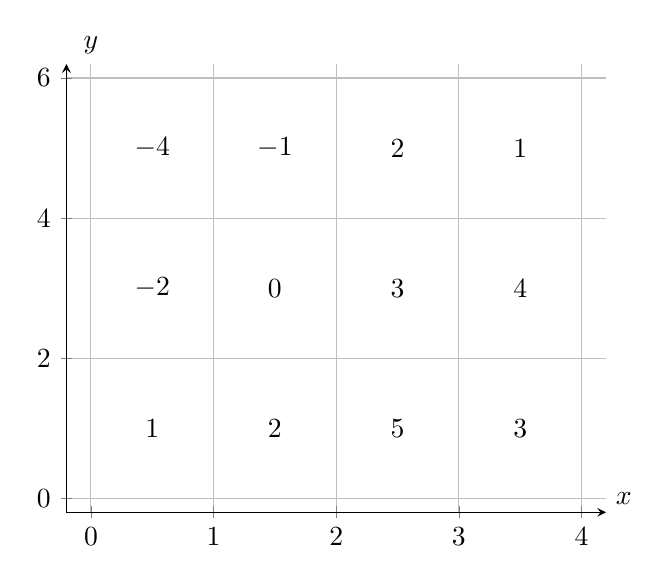
\begin{tikzpicture}
      \begin{axis}
	[xmin=-0.2,
          xmax=4.2,
          ymin=-0.2,
          ymax=6.2,
          axis x line=bottom,
          axis y line=left,
          xlabel=$x$,ylabel=$y$,
          every axis y label/.style={at=(current axis.above origin),anchor=south},
          every axis x label/.style={at=(current axis.right of origin),anchor=west},
	  domain=-1:2,
          clip=false,
	  ytick={0,2,4,6},
	  yticklabels={$0$,$2$,$4$,$6$},
	  xtick={0,1,2,3,4},
	  xticklabels={$0$,$1$,$2$,$3$,$4$},
	  grid = major
	]
	\node at (axis cs: .5,1) {$1$};
        \node at (axis cs: .5,3) {$-2$};
        \node at (axis cs: .5,5) {$-4$};
        
        \node at (axis cs: 1.5,1) {$2$};
        \node at (axis cs: 1.5,3) {$0$};
        \node at (axis cs: 1.5,5) {$-1$};
        
        \node at (axis cs: 2.5,1) {$5$};
        \node at (axis cs: 2.5,3) {$3$};
        \node at (axis cs: 2.5,5) {$2$};
        
        \node at (axis cs: 3.5,1) {$3$};
        \node at (axis cs: 3.5,3) {$4$};
        \node at (axis cs: 3.5,5) {$1$};
      \end{axis}
    \end{tikzpicture}
  \end{image}
  Let
  \[
  R = \{(x,y): \text{$0\le x\le 4$ and $0\le y\le 6$}\}
  \]
  \begin{prompt}
    \begin{align*}
      \Delta x &= \answer{1}\\
      \Delta y &= \answer{2}
    \end{align*}
  \end{prompt}
  \begin{prompt}
    Now, simply add up the $z$-values found in the rectangles that are
    within our region and multiply by $\answer{2}$.
  \end{prompt}
  Compute $\iint_R F(x,y)\d A$.
  \begin{prompt}
    \[
    \iint_R F(x,y) \d A = \answer{28}
    \]
  \end{prompt}
\end{question}


How do we compute a double integral with calculus? We use an
\textit{iterated integral}. At this point we will introduce something
called \textit{Fubini's Theorem}.


\subsection{Fubini's Theorem}

Fubini's Theorem gives us a recipe for computing double integrals. In
this class, we are going to have many different versions of Fubini's
Theorem. The common factor between all of these theorems is that with
each, the ``punch-line'' will be:
\[
\underbrace{\iint_R F(x,y) \d A}_{\text{a double integral}} = \underbrace{\int_?^? \int_?^? F(x,y) \d A}_{\text{an iterated integral}}
\]
where an \textit{iterated integral}\index{iterated integral} is
nothing more than two applications of our familiar friend/foe: the
single integral.


\begin{theorem}[Fubini's Theorem]\index{Fubini's Theorem}
  Let $F$ be continuous on the region
  \[
  R = \{(x,y):\text{$a\le x\le b$ and $c\le y\le d$}\}.
  \]
  Then:
  \begin{align*}
  \iint_R F(x,y) \d A  &= \int_a^b\int_c^d F(x,y)\d y\d x\\
  &=\int_c^d\int_a^b F(x,y)\d x\d y.
  \end{align*}
\end{theorem}

\begin{remark}
  This theorem says \textbf{two} things at once:
  \begin{itemize}
  \item Double integrals can be computed via iterated integrals.
  \item The order of integration can be changed, as long as the bounds
    are changed as well.
  \end{itemize}
\end{remark}


Now let's work some examples:

\begin{example}
  Let $F(x,y) = xy+e^y$. Find the signed volume under $F$ on the region
  \[
  R = \{(x,y):\text{$3\le x\le4$ and $1\le y\le 2$}\}.
  \]
  \begin{image}
    \begin{tikzpicture}
      \begin{axis}%
        [
          tick label style={font=\scriptsize},%axis on top,
	  axis lines=center,
	  view={45}{20},
	  name=myplot,
	  xtick={1,2,3,4},
	  %ytick={5},
	  %ztick={.7,-.7},
	  minor xtick=1,
	  minor ytick=1,
	  ymin=-.1,ymax=2.5,
	  xmin=-.1,xmax=4.5,
	  zmin=-.1, zmax=16,
	  every axis x label/.style={at={(axis cs:\pgfkeysvalueof{/pgfplots/xmax},0,0)},xshift=-1pt,yshift=-4pt},
	  xlabel={\scriptsize $x$},
	  every axis y label/.style={at={(axis cs:0,\pgfkeysvalueof{/pgfplots/ymax},0)},xshift=5pt,yshift=-3pt},
	  ylabel={\scriptsize $y$},
	  every axis z label/.style={at={(axis cs:0,0,\pgfkeysvalueof{/pgfplots/zmax})},xshift=0pt,yshift=4pt},
	  zlabel={\scriptsize $z$},
          colormap/cool
	]        
        \draw [thick,penColor] (axis cs: 3,1,0) -- (axis cs: 3,2,0) -- (axis cs: 4,2,0) -- node [above,pos=.7,black] {\scriptsize $R$} (axis cs: 4,1,0) -- cycle;
        
        \addplot3[domain=0:4.3,,y domain=0:2.1,mesh,samples=13,samples y=18,very thin,z buffer=sort] {x*y+exp(y)};
        
        \addplot3[domain=1:2,%fill=white,
          penColor,very thick,samples=20,samples y=0] ({3},{x},{3*x+exp(x)});
        
        \addplot3[domain=1:2,%fill=white,
          penColor,very thick,samples=20,samples y=0] ({4},{x},{4*x+exp(x)});
        
        \addplot3[domain=3:4,%fill=white,
          penColor,very thick,samples=20,samples y=0] ({x},{1},{1*x+exp(1)});
        
        \addplot3[domain=3:4,%fill=white,
          penColor,very thick,samples=20,samples y=0] ({x},{2},{2*x+exp(2)});
        
        \draw [penColor,dashed,thin] 
	(axis cs: 3,1,0) -- (axis cs: 3,1,5.7)
	(axis cs: 3,2,0) -- (axis cs: 3,2,13.4)
	(axis cs: 4,2,0) -- (axis cs: 4,2,15.4)
	(axis cs: 4,1,0) -- (axis cs: 4,1,6.7);
      \end{axis}
    \end{tikzpicture}
  \end{image}
  \begin{explanation}
    We will compute this integral two different ways. First apply Fubini's Theorem:
    \[
    \iint_R \big(xy+e^y\big) \d A = \int_3^{\answer[given]{4}}\int_{\answer[given]{1}}^{\answer[given]{2}}\big(xy+e^y\big) \d \answer[given]{y} \d \answer[given]{x}
    \]
    Now integrate with respect to $y$, treating $x$ as a constant:
    \begin{align*}
    = \int_{\answer[given]{3}}^{\answer[given]{4}} \eval{\answer[given]{\frac{1}{2}xy^2+e^y}}_{\answer[given]{1}}^{\answer[given]{2}} \d \answer[given]{x} \\
    &= \int_{\answer[given]{3}}^{\answer[given]{4}}\left(\answer[given]{\frac{3}{2}x + e^2-e}\right)\d \answer[given]{x}
    \end{align*}
    Now integrate with respect to $x$, treating $y$ as a constant:
    \begin{align*}
      &= \eval{\answer[given]{\frac{3}{4}x^2 + (e^2-e)x}}_{\answer[given]{3}}^{\answer[given]{4}} \\
      &= \answer[given]{\frac{21}{4}+ e^2-e}.
    \end{align*}

    
  Now let's compute this integral using a \textbf{different order of
  integration.} Write with me,
  \begin{align*}
    \iint_R\big(xy+e^y\big) \d A &= \int_1^{\answer[given]{2}}\int_{\answer[given]{3}}^{\answer[given]{4}}\big(xy+e^y\big)\d \answer[given]{x} \d \answer[given]{y} \\
    &= \int_{\answer[given]{1}}^{\answer[given]{2}}\eval{\answer[given]{\frac{1}{2}x^2y+xe^y}}_{\answer[given]{3}}^{\answer[given]{4}}\d \answer[given]{y}\\
    &= \int_{\answer[given]{1}}^{\answer[given]{2}}\left(\answer[given]{\frac{7}{2}y+e^y}\right)\d \answer[given]{y}\\
    &= \eval{\answer[given]{\frac{7}{4}y^2+e^y}}_{\answer[given]{1}}^{\answer[given]{2}}\\
    &=\answer[given]{\frac{21}{4}+e^2-e}.
  \end{align*}
  Note our answers are \textbf{the same} regardless of the order of
  integration.
  \end{explanation}
\end{example}

In our next example, we will see that it is sometimes easier to apply
Fubini's Theorem and integrate with respect to one variable instead of
the other.

\begin{example}
  Let $F(x,y) = xe^{xy}$. Find the signed volume under $F$ on the region
  \[
  R = \{(x,y):\text{$0\le x\le 1$ and $0\le y\le 1$}\}.
  \]
  \begin{image}
    \begin{tikzpicture}
      \begin{axis}%
        [
          tick label style={font=\scriptsize},%axis on top,
	  axis lines=center,
	  view={120}{20}, %% rotate around / up and down
	  name=myplot,
	  ymin=-.1,ymax=1.1,
	  xmin=-.1,xmax=1.1,
	  zmin=-.1, zmax=3,
	  every axis x label/.style={at={(axis cs:\pgfkeysvalueof{/pgfplots/xmax},0,0)},xshift=-1pt,yshift=-4pt},
	  xlabel={\scriptsize $x$},
	  every axis y label/.style={at={(axis cs:0,\pgfkeysvalueof{/pgfplots/ymax},0)},xshift=5pt,yshift=-3pt},
	  ylabel={\scriptsize $y$},
	  every axis z label/.style={at={(axis cs:0,0,\pgfkeysvalueof{/pgfplots/zmax})},xshift=0pt,yshift=4pt},
	  zlabel={\scriptsize $z$},
          colormap/cool
	]        
        \draw [ultra thick,penColor] (axis cs: 0,0,0) -- (axis cs: 1,0,0) -- (axis cs: 1,1,0) -- (axis cs: 0,1,0) -- cycle;
        
        \node at (axis cs: .5,.5,0) {\scriptsize $R$};
        
        \addplot3[domain=0:1,,y domain=0:1,mesh,samples=13,samples y=18,very thin,z buffer=sort] {x*exp(x*y)};
        
        \addplot3[domain=0:1,%fill=white,
          penColor,very thick,samples=20,samples y=0] ({1},{x},{exp(x)});
        
        \addplot3[domain=0:1,%fill=white,
          penColor,very thick,samples=20,samples y=0] ({0},{x},{0});
        
        \addplot3[domain=0:1,%fill=white,
          penColor,very thick,samples=20,samples y=0] ({x},{0},{x});
        
        \addplot3[domain=0:1,%fill=white,
          penColor,very thick,samples=20,samples y=0] ({x},{1},{x*exp(x)});
       \end{axis}
    \end{tikzpicture}
  \end{image}
  \begin{explanation}
    Let's first compute:
    \[
    \int_0^1 \int_0^1 x e^{xy} \d x \d y
    \]
    As we will see, this integral will require three tricks. To
    integrate with respect to $x$, you can use integration by parts:
    \begin{align*}
      \int_0^1 \int_0^1 x e^{xy} \d x \d y &= \int_0^1 \eval{\answer[given]{\frac{xe^{xy}}{y}-\frac{e^{xy}}{y^2}}}_0^1\d y\\
      &= \int_0^1 \left(\frac{e^{y}}{y}-\frac{e^y}{y^2} + \frac{1}{y^2}\right)\d y
    \end{align*}
    Now we notice that this is an improper integral!
    We must therefore compute
    \[
    \lim_{b\to\answer[given]{0}}\int_{\answer[given]{b}}^{\answer[given]{1}} \left(\answer[given]{\frac{e^{y}}{y}-\frac{e^y}{y^2} + \frac{1}{y^2}}\right)\d y
    \]
    Now we must integrate with respect to $y$. This is also
    tricky. Our second trick is to rewrite our current integrand as
    \[
    \frac{y e^y - \left(\answer[given]{e^y -1}\right)}{y^2}
    \]
    and now ``see'' that this results from the quotient rule being
    applied to
    \[
    \frac{e^y-\answer[given]{1}}{y}.
    \]
    So now we must compute:
    \begin{align*}
      \lim_{b\to \answer[given]{0}}\eval{\frac{e^y-1}{y}}_{\answer[given]{b}}^{\answer[given]{1}} &= \lim_{\answer[given]{b}\to \answer[given]{0}}\left(\answer[given]{\frac{e^1-1}{1}-\frac{e^b-1}{b}}\right)\\
      &= \frac{e^1-1}{1}-\lim_{b\to 0}\answer[given]{\frac{e^b-1}{b}}.
    \end{align*}
    Now, for our third trick, we'll use L'H\^opital's rule. Note that
    the numerator and denominator both go to zero and are
    differentiable, so this is OK.
    \begin{align*}
    \lim_{b\to 0}\frac{e^b-1}{b} &= \lim_{b\to 0}\answer[given]{\frac{e^b}{1}}\\
    &= \answer[given]{1}.
    \end{align*}
    So putting this all together, we have
    \[
    \int_0^1 \int_0^1 x e^{xy} \d x \d y = \answer[given]{e-2}
    \]
    Whew. This was hard!


    Now use Fubini's Theorem and integrate with respect to $y$ first!
    Fubini's theorem says:
    \[
    \int_0^1 \int_0^1 x e^{xy} \d x \d y =  \int_0^1 \int_0^1 x e^{xy} \d y \d x
    \]
    provided you switch the order of integration. Note, in this case
    the limits of integration for both $x$ and $y$ are the same, but
    we \textit{did} switch them. Let's get on with it! Write with me:
    \begin{align*}
      \int_0^1 \int_0^1 x e^{xy} \d y \d x &= \int_0^1 \eval{\answer[given]{e^{xy}}}_0^1\d x\\
      &= \int_0^1 \left(\answer[given]{e^x - 1}\right) \d x \\
      &= \eval{\answer[given]{e^x - x}}_0^1\\
      &= \answer[given]{e-2}
    \end{align*}
    Man alive! That was easy! Note, we get the same final answer
    regardless of the order of integration. Thank-you Fubini!
  \end{explanation}
\end{example}



\section{Triple integrals}

Using a similar technique to how we made boxes to define double
integrals, we can make four-dimensional \textit{boxes} to define a
triple integral that computes the signed
\link[hypervolume]{http://en.wikipedia.org/wiki/Four-dimensional_space}
bounded by a
\link[hypersurface]{http://en.wikipedia.org/wiki/Four-dimensional_space}
and a three-dimensional region.
\[
\iiint_R F(x,y,z) \d V = \lim_{\substack{\l\to\infty\\ m\to\infty\\ n\to\infty}}
\sum_{k=1}^n
\sum_{j=1}^m
\sum_{i=1}^\l
F(x^*_i,y^*_j,z_k^*)\Delta x\Delta y\Delta z
\]
How do we compute a triple integral with calculus? We use our second
version of Fubini's Theorem. This time, it will say something like:

\[
\underbrace{\iiint_R F(x,y,z) \d V}_{\text{a triple integral}} = \underbrace{\int_?^? \int_?^? \int_?^? F(x,y,z) \d V}_{\text{an iterated integral}}
\]

\begin{theorem}[Fubini's Theorem]\index{Fubini's Theorem}
  Let $F$ be continuous on the region
  \[
  R = \{(x,y,z):\text{$a\le x\le b$, $c\le y\le d$, $p\le z\le q$}\}.
  \]
  Then:
  \[
  \iiint_R F(x,y,z) \d V  = \int_a^b\int_c^d\int_p^q F(x,y,z)\d z \d y\d x.
  \]
  Here, all \textit{six} combinations of orders of integration will
  work, and be equal, provided that the bounds are changed
  appropriately.
\end{theorem}

\begin{remark}
  Note that when computing a triple iterated integral, after the
  innermost integral is evaluated, you are now working with a double
  iterated integral.
\end{remark}






\begin{question}
  Let $F$ be a continuous function on the region $R$.
  \begin{align*}
    \int_a^b\int_c^d\int_p^q &F(x,y,z)\d z \d y\d x \\
    &= \int_{\answer{p}}^{\answer{q}}\int_a^{\answer{b}}
    \int_{\answer{c}}^d F(x,y,z)\d \answer{y} \d \answer{x} \d \answer{z}
  \end{align*}
  \begin{question}
    \begin{hint}
      \[
      \int_a^b f(x) \d x = - \int_b^a f(x) \d x
      \]
    \end{hint}
    \begin{align*}
      \int_a^b\int_c^d\int_p^q &F(x,y,z)\d z \d y\d x \\
      &= \int_{\answer{c}}^{d}
    \int_{\answer{b}}^{a}\int_{\answer{q}}^{\answer{p}}
    F(x,y,z)\d \answer{z} \d \answer{x} \d \answer{y}
    \end{align*}
  \end{question}
\end{question}

Let's do an example.


\begin{example}
  Let $F(x,y,z) = \cos(x-y)\sin(z)$. Find the signed hypervolume ``under'' $F$ on the region
  \[
  R = \{(x,y):\text{$0\le x\le \pi$, $0\le y\le \pi$, and $0\le z\le \pi$}\}.
  \]
  \begin{explanation}
    First apply Fubini's Theorem to convert the triple integral into an iterated integral:
    \[
    \iiint_R F(x,y,z) \d V =\int_{\answer[given]{0}}^{\answer[given]{\pi}}\int_{\answer[given]{0}}^{\answer[given]{\pi}}\int_{\answer[given]{0}}^{\answer[given]{\pi}} \answer[given]{\cos(x-y)\sin(z)} \d x \d y \d z
    \]
    Now integrate with respect to $x$:
    \begin{align*}
      &= \int_{\answer[given]{0}}^{\answer[given]{\pi}}\int_{\answer[given]{0}}^{\answer[given]{\pi}}\eval{\answer[given]{\sin(x-y)\sin(z)}}_{\answer[given]{0}}^{\answer[given]{\pi}}\d y \d z \\
      &= \int_{\answer[given]{0}}^{\answer[given]{\pi}}\int_{\answer[given]{0}}^{\answer[given]{\pi}}\left(\answer[given]{\sin(\pi-y)\sin(z) + \sin(y)\sin(z)}\right)\d y \d z 
    \end{align*}
    Now integrate with respect to $y$:
    \begin{align*}
      &= \int_{\answer[given]{0}}^{\answer[given]{\pi}}\eval{\answer[given]{\cos(\pi-y)\sin(z) -\cos(y)\sin(z)}}_{\answer[given]{0}}^{\answer[given]{\pi}} \d z\\
      &= \int_{\answer[given]{0}}^{\answer[given]{\pi}}\answer[given]{4\sin(z)} \d z
    \end{align*}
    Finally integrate with respect to $z$:
    \begin{align*}
      &= \eval{\answer[given]{-4\cos(z)}}_{\answer[given]{0}}^{\answer[given]{\pi}} \\
      &= \answer[given]{8}
    \end{align*}
  \end{explanation}
\end{example}

We've just begun our journey with multiple integrals. Next, we'll think about
more complex regions! For some interesting extra reading check out:
\begin{itemize}
\item \link[\textit{Three Aspects of Fubini's Theorem}, J.\ C.\ Fisher and
  J.\ Shilleto, Mathematics Magazine, February
  1986]{http://www.jstor.org/stable/2690017}.
\item \link[\textit{Visualizing Leibniz's Rule}, M.\ Frantz, Mathematics
      Magazine, April 2001]{http://www.jstor.org/stable/2690632}.
\end{itemize}
\end{document}
